\title{Structure-oriented singular value decomposition for random noise attenuation of seismic data}
\renewcommand{\thefootnote}{\fnsymbol{footnote}}

\author{Shuwei Gan\footnotemark[1], Yangkang Chen\footnotemark[2], Shaohuan Zu \footnotemark[1], Shan Qu\footnotemark[1] and Wei Zhong \footnotemark[1]}

\address{
\footnotemark[1] State Key Laboratory of Petroleum Resources and Prospecting \\
China University of Petroleum \\
Fuxue Road 18th\\
Beijing, China, 102200 \\
gsw19900128@126.com\\
\footnotemark[2]Bureau of Economic Geology \\
John A. and Katherine G. Jackson School of Geosciences \\
The University of Texas at Austin \\
University Station, Box X \\
Austin, TX 78713-8924 \\
ykchen@utexas.edu
}

\lefthead{Gan et al.}
\righthead{Structure-oriented SVD}
\maketitle

\begin{abstract}
Singular value decomposition (SVD) can be used both globally and locally to remove random noise in order to improve the signal-to-noise ratio (SNR) of seismic data. However, they can only be applied to seismic data with simple structure such that there is only one dip component in each processing window. We introduce a novel denoising approach that utilizes a structure-oriented SVD and this approach can enhance seismic reflections with continuous slopes. We create a third dimension for a 2D seismic profile by using the plane-wave prediction operator to predict each trace from its neighbour traces and apply SVD along this dimension. The added dimension is equal to flattening the seismic reflections within a neighbouring window. The third dimension is then averaged to decrease the dimension. We use two synthetic examples with different complexities and one field data example to demonstrate the performance of the proposed structure-oriented SVD. Compared with global and local SVDs, and $f-x$ deconvolution, the structure-oriented SVD can obtain much clearer reflections and preserve more useful energy. 
\end{abstract}

\section{Keywords}
Singular value decomposition, random noise attenuation, global SVD, local SVD, structure-oriented SVD

\section{Introduction}
The attenuation of random noise is an important subject in seismic data processing. The enhanced seismic signals with higher signal-to-noise ratio (SNR) can help interpreters to make more accurate decisions. There are generally four different categories of random noise attenuation approaches that exist in the exploration geophysics literatures. The first is based on the predictive property of useful signals in small spatial-temporal windows, such as $f-x$ deconvolution \cite[]{canales,yangkang2014}, $f-x-y$ prediction filtering \cite[]{yanghua1999,yanghua2002}, $t-x$ prediction error filtering \cite[]{abma1995}, and $f-x$ non-stationary polynomial fitting \cite[]{guochang20112}. \new{\cite{wencheng2015asa} proposed a novel trace-by-trace random noise attenuation approach based on the predictable spectral components property of useful seismic reflections using regularized non-stationary autoregression \cite[]{fomel20132}. This approach does not require the spatial coherency assumption and has the potential to be widely used to denoise microseismic signal, the SNR of which is very low.}  The second is based on the statistical property of seismic profile, such as the mean filter \cite[]{nlm}, median filter \cite[]{yike2013,yangkang2014svmf,yangkang2014nmo}. The third is based on extracting the principal components of seismic data, such as multichannel singular spectrum analysis (MSSA) \cite[]{mssa,yangkang2015} and EMD based approaches \cite[]{yangkang2014emdsum}. This type of approach is also related with those rank-reduction based approaches, eigenimage-based approaches. The fourth is based on a transformed domain thresholding strategy \cite[]{curvelet,seislet,yangkang20142}. The transform operator can be a fixed-basis sparsity-promoting transform, and can also be an adaptively-learned dictionary, while the fixed-basis transform enjoys better efficiency and learning-based dictionary enjoys better adaptivity. Apart from those aforementioned one-step noise attenuation, \cite{yangkang2015ortho} proposed a two-step approach for retrieving the lost useful signals from the noise section, which can be seen as the residual random noise attenuation. 


\cite{freire1988svdsnr} proposed to carry out rank reduction of seismic images in the $t-x$ domain via singular value decomposition (SVD). They applied SVD to the seismic data matrix and extracted the first singular value in order to remove random noise based on the assumption that the seismic data with only horizontal events have a rank of one. We refer to this method as the global SVD (GSVD), because this SVD method does not require to be implemented in small windows. The GSVD does not require regularly sampled data because no convolutional operator is used. As long as the seismic profiles are composed with horizontal events, GSVD can obtain a good denoising performance. However, the seismic profiles do not necessarily meet the requirement that there are no dipping events. For those complex profiles, GSVD cannot be applied. \cite{freire1988svdsnr} also demonstrated that the GSVD is actually equivalent to Karhunen-Loeve (KL) (or principal component transformation) approach \cite[]{jones1987}. Because of the horizontal-energy selective property of GSVD, \cite{milton2009} proposed to use GSVD filtering to remove dipping interference, such as ground-rolls.  

The $f-x$ domain rank reduction approaches are independent from dip, and therefore, do not require flattening. They require an eigen-decomposition of the spectral matrix of data, which is connected with Cadzow filtering \cite[]{cadzow1988} and multichannel singular spectrum analysis (MSSA) \cite[]{vautard1992,mssa}.
Although MSSA and Cadzow filtering are equivalent, they come from different signal analysis subfields. Cadzow filtering was proposed to denoise images, whereas MSSA was proposed to decompose time series arising in the study of dynamical systems \cite[]{oropeza2010}. Cadzow filtering and MSSA are also referred to as the $f-x$ SVD (FXSVD). For FXSVD, the eigen-decomposition of spectral matrix is usually done by applying an SVD to a pre-constructed (block) Hankel matrix. However, this type of methods depends on the low-rank property of seismic data, in other words, the seismic profile should contain few linear events (2D) or few plane-wave components (3D). The low-rank and linear-events assumptions of the FXSVD are not always met, which enforces the FXSVD to be implemented in local processing windows. The division of local windows and decision of rank value, however, are sometimes an empirical and user-unfriendly process.

In this paper, we propose a novel SVD approach for enhancing useful reflections by removing random noise. The novel SVD is implemented obeying the structural information.
We first flatten the seismic reflections according to the local slopes by trace prediction. In the flattened domain, we apply a GSVD to horizontal events in order to remove random noise. The flattened traces are then transformed back to the original structural shape by stacking the traces in the flattened domain. We refer to the proposed novel SVD denoising approach as structure-oriented SVD (SOSVD). The SOSVD does not require local processing windows as LSVD and FXSVD do, and it can distinguish signal and noise better than GSVD. Flattened events make the largest singular value components mainly correspond to useful events, which are much easier to be separated. However, GSVD may not be applied to flattened events. 

We organize the paper as follows: we first introduce the well-known GSVD, LSVD along with dip steering, and the theoretical aspects of SOSVD. \new{A brief review of the basic theory of the commonly used $f-x$ deconvolution is also provided in the appendix.} We then \old{compare}\new{apply} three different SVDs and \old{commonly used} $f-x$ deconvolution onto three different synthetic examples (with increasing complexity) and one field data example that comes from the \old{Gulf of Mexico}\new{North Sea}, and compare their performances. The comparisons show that the SOSVD can obtain much better performance in removing noise and preserving useful signals. 

\section{Theory}
\subsection{Noise attenuation using SVD}
2D seismic data can be expressed as a data matrix $\mathbf{D}$ ($M\times N$), consisting of $N$ traces and $M$ time samples. The SVD of the data matrix $\mathbf{D}$ can be expressed as:
\begin{equation}
\label{eq:svd}
\mathbf{D}=\mathbf{U\Sigma V}^T.
\end{equation}
Here, $\mathbf{U}$ is composed of the eigenvectors of $\mathbf{DD}^T$. $\mathbf{V}$ is composed of the eigenvectors of $\mathbf{D}^T\mathbf{D}$. $\mathbf{\Sigma}$ is a diagonal matrix composed of the decreasing singular values. Let us denote $\mathbf{U}$, $\mathbf{\Sigma}$, and $\mathbf{V}$ in the following form:
\begin{equation}
\label{eq:svdu}
\begin{array}{l}
\mathbf{U}=[u_1,u_2,\cdots,u_r],\\
\mathbf{\Sigma}=diag(\sigma_1,\sigma_,\cdots,\sigma_r),\\
\mathbf{V}=[v_1,v_2,\cdots,v_r],
\end{array}
\end{equation}
where $r$ is the rank of $\mathbf{D}$. The vectors $\mathbf{u}_k$ and $\mathbf{v}_k$ are also called the propagation vectors and the eigen-wavelets, respectively \cite[]{vrabie2004}. The singular values $\sigma_k$ are sorted such that $\sigma_1\ge\sigma_2\ge\cdots\ge\sigma_r$. They can be obtained by calculating the positive square roots of the eigenvalues of the data covariance matrix $\mathbf{D}\mathbf{D}^T$.

Equation \ref{eq:svd} can be expressed as:
\begin{equation}
\label{eq:svd2}
\mathbf{D} = \sum_{k=1}^{r}\lambda_k\mathbf{u}_k\mathbf{v}^T_{k},
\end{equation}
where $\mathbf{u}_k\mathbf{v}^T$ is the rank-one matrix called the $k$th eigenimage of $\mathbf{D}$. Thus, from equation \ref{eq:svd2}, the seismic image can be decomposed into $r$ eigenimages, %Matrix $\mathbf{D}$ can be decomposed into $r$ parts, 
the energy of which corresponds to the value of each element in matrix $\mathbf{\Sigma}$. 

We can remove the random noise in seismic data in order to enhance the seismic reflections by only selecting the first several eigenimages \cite[]{freire1988svdsnr}:
\begin{equation}
\label{eq:svddenoise}
\hat{D}_{svd} = \sum_{k=1}^{p} \sigma_k\mathbf{u}_k\mathbf{v}_k^T.
\end{equation}

Random noise attenuation approach by SVD utilizes the property that useful seismic signals are horizontally coherent to separate signal and noise. %Let $\mathbf{D}$ denotes the seismic profile with $N$ traces and $M$ temporal samplings. 
The decomposition is based on the criterion of horizontal coherency. The energy of coherent signals lays in the first several parts of the decomposition, which is represented by the value of bigger values in $\mathbf{\Sigma}$. For seismic data, the horizontal coherent part corresponds to useful signal while random noise or coherent dipping events are not horizontally coherent. Thus, by choosing the first several elements in $\mathbf{\Sigma}$ and making the others equal to zero, we can remove the noise and enhance seismic data quality. SVD acts as a data-driven, low-pass filter by rejecting highly uncorrelated traces \cite[]{bekara2007}. Here, we refer to those denoising approaches that simply apply SVD to the original seismic data in order to remove random noise as global SVD (GSVD).

\subsection{Dip steering and local SVD}
Supposing the events in a processing window have one slope, dip steering algorithm aims to flatten the dipping events by shifting each trace such that the flattened events are suitable for applying a GSVD based denoising approach, as shown in equation \ref{eq:svddenoise}. This flattening strategy is called dip steering \cite[]{bekara2007}. After removing noise, applying an inverse flattening to the data in the processing window can obtain the denoised data. We refer to those denoising approaches that apply a GSVD in the dip-steering flattened domain as local SVD (LSVD).
The time shifts for each trace in order to flatten the events are obtained by selecting the time delays that can maximize cross-correlation between each trace and a reference trace.  
\begin{equation}
\label{eq:steer}
\tau_n = \arg\max_{\tau} \sum_{m=\min(1-\tau,1)}^{\max(M_w,M_w-\tau)} r(m)d(m+\tau,n),
\end{equation}
where $\tau_n$ is the optimal time shift for $n$th trace in the processing window, $M_w$ denotes the number of time samples in the processing window and $r(m)$ denotes the $m$th sample of the reference trace and $d(m,n)$ denotes the data value in $m$th sample and $n$th trace.
$\tau_n>0$ corresponds to shifting trace downward with respect to the reference trace, and $\tau_n<0$ corresponds to shifting trace upward.

As can be seen from the equation \ref{eq:steer}, the selection of reference trace is crucial for the effectiveness of LSVD. It can be chosen as random trace in the processing window if the noise level is not high, or can be chosen as a stacked trace after normal-moveout (NMO) of common-midpoint gathers. \cite{bekara2007} proposed an iterative strategy for selecting the optimal reference trace stating that the resulting shifted traces are stacked after each cross-correlation pass for updating the new reference traces and the process of cross-correlation, shifting, and stacking is repeated until the process converges.
Figure \ref{fig:dn,dh,dhc,dc} shows a demonstration for dip steering and the processes of LSVD. Figure \ref{fig:dn} is the original noisy dipping event. Figure \ref{fig:dh} denotes the flattened event after forward dip steering. Figure \ref{fig:dhc} shows the LSVD denoised result by choosing only one singular value. The final denoised result after inverse dip steering on Figure \ref{fig:dhc} is shown in Figure \ref{fig:dc}. The time shifts after the optimizing equation \ref{eq:steer} are shown in Figure \ref{fig:shift}. The reference trace is simply chosen as the first trace of the original data, as shown in Figure \ref{fig:dn}.

\AtEndDocument{
\begin{figure}[htb!]
\centering
\subfigure[]{\includegraphics[width=0.45\columnwidth,height=0.4\columnwidth]{dipsteer/Fig/dn}
	\label{fig:dn}}
\subfigure[]{\includegraphics[width=0.45\columnwidth,height=0.4\columnwidth]{dipsteer/Fig/dh}
	\label{fig:dh}}
\subfigure[]{\includegraphics[width=0.45\columnwidth,height=0.4\columnwidth]{dipsteer/Fig/dhc}
	\label{fig:dhc}}
\subfigure[]{\includegraphics[width=0.45\columnwidth,height=0.4\columnwidth]{dipsteer/Fig/dc}
	\label{fig:dc}}
\caption{Demonstration for dip steering and LSVD. (a) Noisy dip reflector. (b) Flattened event using dip steering. (c) SVD denoised result by selecting only one eigen-image. (d) Denoised data after inverse dip steering.}
\label{fig:dn,dh,dhc,dc}
\end{figure}

\begin{figure}[htb!]
\centering
\includegraphics[width=0.85\columnwidth,height=0.8\columnwidth]{dipsteer/Fig/shift}
\caption{Time shifts for each trace for the forward dip steering as shown in Figure \ref{fig:dn,dh,dhc,dc} (reference trace selected as the left trace in Figure \ref{fig:dn}).}
\label{fig:shift}
\end{figure}
}

\subsection{Structure-oriented SVD}
The structure-oriented SVD (SOSVD) refers to two processes: flattening along the local structure in a local  spatial window and applying GSVD in the flattened local spatial window. The procedures can be summarized as:
\begin{equation}
\label{eq:proc}
\mathbf{D} \rightarrow \mathbf{D}_j^R (j=1,2,\cdots,N) \rightarrow \overline{\mathbf{D}}_j^R \rightarrow \overline{\overline{D}}_j^R \rightarrow \mathbf{d}_j \rightarrow \hat{\mathbf{D}}_{sosvd}.
\end{equation}

Here, $\mathbf{D}_j^R$ denotes the $j$th spatial window (corresponding to $j$th trace) with a radius of $R$, $\overline{\mathbf{D}}_j^R$ denotes the flattened local spatial window, $\overline{\overline{D}}_j^R$ denotes the SVD denoised local spatial window, $\mathbf{d}_j$ denotes the averaged local spatial window, and $\hat{\mathbf{D}}_{sosvd}$ denotes the output data using SOSVD.

As we can see from the workflow, the key step that distinguishes SOSVD with other types of SVD approaches is the flattening in the local spatial window. The flattening corresponds to applying a flattening operator to the data (here we use a prediction operator according to local slope) so that the output data have horizontal events:
\begin{equation}
\label{eq:flatten}
 \mathbf{P}_j \mathbf{D}_j^R= \overline{\mathbf{D}}_j^R.
\end{equation}
where $\mathbf{P}_j$ is the $j$th flattening operator. Here, the flattening operator is chosen as a plane-wave prediction operator related with the local slope. 
Equation \ref{eq:flatten} has the following detailed form:
\begin{equation}
\label{eq:detail}
\begin{split}
& \left[
\begin{array}{cccccc}
\mathbf{P}_{(1,j)\rightarrow(1+R,j)}(\sigma_{1,j}) &  & & & & \\
 &  & \ddots & & & \\
 &  & & \mathbf{P}_{(1+R,j)\rightarrow(1+R,j)}(\sigma_{1+R,j}) & & \\
 &  & & & \ddots & \\
 &  & & & & \mathbf{P}_{(1+2R,j)\rightarrow(1+R,j)}(\sigma_{1+2R,j})\\
\end{array}
\right]\\
&[\mathbf{d}_{1,j},\cdots,\mathbf{d}_{1+R,j}, \cdots, \mathbf{d}_{1+2R,j}]\\
&=[\overline{\mathbf{d}}_{1,j},\cdots,\overline{\mathbf{d}}_{1+R,j}, \cdots, \overline{\mathbf{d}}_{1+2R,j}]. 
\end{split}
\end{equation}
Here, $\mathbf{P}_{(i,j)\rightarrow(k,j)}(\sigma_{i,j})$ denotes the prediction operator from trace $i$ to trace $k$ in $j$th spatial window, which is connected with the local slope of $i$th trace.  Prediction of a trace consists of shifting the original trace along dominant event slopes \cite[]{fomel2010painting}.  
Prediction of a trace from a distant neighbour can be accomplished by simple recursion \cite[]{liuyang2010}, i.e., predicting trace $k$ from trace $1$ is simply
\begin{equation}
\label{eq:recur}
\mathbf{P}_{(1,j)\rightarrow(k,j)} (\sigma_{1,j})= \mathbf{P}_{(k-1,j)\rightarrow(k,j)}(\sigma_{k-1,j})\cdots\mathbf{P}_{(2,j)\rightarrow(3,j)}(\sigma_{2,j})\mathbf{P}_{(1,j)\rightarrow(2,j)}(\sigma_{1,j}).
\end{equation}

The prediction operator is a numerical solution of the local plane differential equation 
\begin{equation}
\label{eq:plane}
\frac{\partial P}{\partial x} + \sigma \frac{\partial P}{\partial t} = 0,
\end{equation}
for local plane wave propagation in the $x$ direction. 

The dominant slopes are estimated by solving the following least-square minimization problem using regularized least-squares optimization:
\begin{equation}
\label{eq:mini}
\hat{\mathbf{\sigma}} = \arg\min_{\sigma} \parallel \mathbf{W}(\sigma)\mathbf{D} \parallel_2^2,
\end{equation}
where \old{$\mathbf{D}$}\new{$\mathbf{W}$} is the destruction operator defined as 

\begin{displaymath} 
\mathbf{W} = \left[
\begin{array}{ccccc} 
\mathbf{I} & 0 & 0 & \cdots & 0\\
-\mathcal{\mathbf{P}}_{1\rightarrow 2} &\mathbf{I} & 0 &\cdots &0\\
0 &-\mathcal{\mathbf{P}}_{2\rightarrow 3} & \mathbf{I} & \cdots & 0 \\
\cdots & \cdots & \cdots & \cdots & \cdots \\
0& 0 & \cdots & - \mathcal{\mathbf{P}}_{N-1\rightarrow N} & \mathbf{I}
\end{array}\right]\;, 
\end{displaymath}
where $\mathbf{I}$ stands for the identity operator, and $\mathcal{\mathbf{P}}_{i\rightarrow k}$ describes prediction of trace $k$ from trace $i$ (same as the previous version $\mathbf{P}_{(i,j)\rightarrow(k,j)}(\sigma_{i,j})$ except for not in a specific spatial window). The optimization approach as shown in equation \ref{eq:mini} for obtaining local slope estimation is called plane wave destruction (PWD) \cite[]{fomel2002pwd}.

\section{Examples}
In this section, we first use two synthetic examples with different complexities. Then a field data example is presented for better demonstration of the proposed approach. \new{For all the three examples, we compare the denoising performances for GSVD, LSVD,SOSVD, and the commonly used $f-x$ deconvolution. A brief review of the theory of $f-x$ deconvolution is provided in the appendix.}

The first synthetic example is a simple seismic profile that has hyperbolic events. It is generated from the SeismicLab library. The clean data and noisy data with simulated Gaussian white noise are shown in Figure \ref{fig:clean,noisy}. There are three hyperbolic events in the synthetic data. Two events have small slopes and the other one has high slope. The denoised results using GSVD, LSVD, and SOSVD are shown in Figures \ref{fig:hyper-gsvd}, \ref{fig:hyper-lsvd}, and \ref{fig:hyper-svd}, respectively. As a reference, we also show the denoised result using $f-x$ deconvolution in Figure \ref{fig:hyper-fx}. From the comparison of denoised results shown in Figure \ref{fig:hyper-gsvd,hyper-lsvd,hyper-fx,hyper-svd}, we can initially conclude that the GSVD removes the least noise, there are some damages to the events for LSVD, $f-x$ deconvolution does a little damage to the dipping hyperbolic event, and the denoised result using the proposed SOSVD obtains a nearly perfect result. The removed noise sections are shown in Figure \ref{fig:hyper-n-gsvd,hyper-n-lsvd,hyper-n-fx,hyper-n-svd}. From the noise sections, we can confirm the observation made from the denoised results shown in Figure \ref{fig:hyper-gsvd,hyper-lsvd,hyper-fx,hyper-svd}. The GSVD cannot remove too much random noise because we cannot remove too many eigen images, otherwise the damages to useful events are very large. The GSVD causes some damages to the steep event, LSVD causes some damages to areas that have conflicting slopes, $f-x$ deconvolution causes damages to both steep event and more horizontal events. There are nearly no coherent signals lost in the noise section for the proposed SOSVD.

The second synthetic example is a linear-event section. Figure \ref{fig:complex-clean,complex-noisy} shows the clean and noisy data. There are one horizontal and three dipping events in this section. Two of the dipping events cross with each other. After using the GSVD, LSVD, $f-x$ deconvolution, and the proposed SOSVD, we obtain four denoised sections, as shown in Figure \ref{fig:complex-gsvd,complex-lsvd,complex-fx,complex-svd}. The GSVD still does a bad job because of the dipping events. The LSVD seems to cause more damages to the useful events than the previous example because almost in each processing window there are more than one slopes, which makes the dip steering strategy fail. $f-x$ deconvolution damages both horizontal and dipping events. The proposed SOSVD removes the most noise and preserves the useful energy best. From the noise sections as shown in Figure \ref{fig:complex-n-gsvd,complex-n-lsvd,complex-n-fx,complex-n-svd}, we conclude that the SOSVD gets an excellent performance except for small damage to the crossing point of the original noisy data. The damage for the crossing point comes from the fact that the PWD algorithm cannot obtain a precise slope estimation in the region and thus causes the flattening along the structure more difficult. \new{In fact, the only disadvantage of the proposed approach is the incapability to handle crossing seismic events. The crossing points will appear in the noise section. The problem can be handled by slope-separated processing using the same approach. However, as a byproduct, the proposed approach may has potential to be used as a diffraction detector, which will be helpful for other important tasks in seismic data processing and imaging. This topic regarding to the crossing point may be the subject of future investigation.}
 
The third example is a field data example. This example is a part extracted from a 3D North Sea data \cite[]{lomask2006,fomel2010painting}.  The original image is shown in Figure \ref{fig:field-noise}. As we can see, the seismic data contain a lot of \old{in-continuous}\new{dis-continuous} events caused by a low SNR, which makes the interpretation and evaluation of the useful signals impossible. After using GSVD, LSVD, $f-x$ deconvolution and SOSVD, we obtain four denoised sections that are shown in Figure \ref{fig:field-gsvd,field-lsvd,field-fx,field-svd}. It's obvious that GSVD and LSVD both cause some damages to the useful signals. Although $f-x$ deconvolution preserves the useful reflections well, there seems no improvement for SNR of the data. By using SOSVD, we can obtain a very good denoised image (Figure \ref{fig:field-svd}). The image becomes clean and seismic reflections becomes continuous, which is beneficial for the following interpretation. From the noise sections shown in Figure \ref{fig:field-n-gsvd,field-n-lsvd,field-n-fx,field-n-svd}, we can get the similar conclusion that  SOSVD preserves the most useful energy while removing the most noise.

\AtEndDocument{ 
\begin{figure}[htb!]
\centering
\subfigure[]{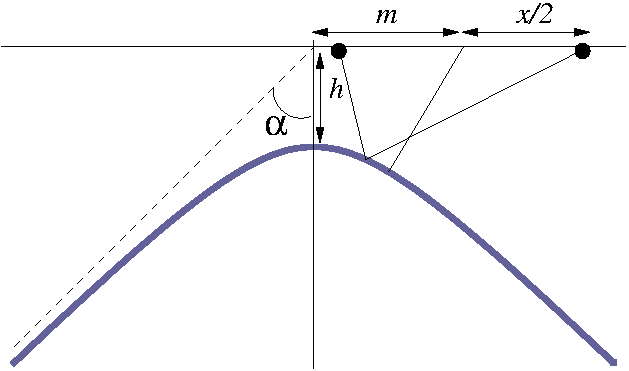
\includegraphics[width=0.45\columnwidth,height=0.4\columnwidth]{hyper/Fig/hyper}
	\label{fig:hyper}}
\subfigure[]{\includegraphics[width=0.45\columnwidth,height=0.4\columnwidth]{hyper/Fig/hyper-noise}
	\label{fig:hyper-noise}}
\caption{Hyperbolic-events synthetic seismic profile. (a) Clean data. (b) Noisy data.}
\label{fig:clean,noisy}
\end{figure}

\begin{figure}[htb!]
\centering
\subfigure[]{\includegraphics[width=0.45\columnwidth,height=0.4\columnwidth]{hyper/Fig/hyper-gsvd}
	\label{fig:hyper-gsvd}}
\subfigure[]{\includegraphics[width=0.45\columnwidth,height=0.4\columnwidth]{hyper/Fig/hyper-lsvd}
	\label{fig:hyper-lsvd}}
\subfigure[]{\includegraphics[width=0.45\columnwidth,height=0.4\columnwidth]{hyper/Fig/hyper-fx}
	\label{fig:hyper-fx}}
\subfigure[]{\includegraphics[width=0.45\columnwidth,height=0.4\columnwidth]{hyper/Fig/hyper-svd}
	\label{fig:hyper-svd}}
\caption{Comparison of denoised data for the hyperbolic-events synthetic example. (a) Using GSVD. (b) Using LSVD. (c) Using $f-x$ deconvolution. (d) Using SOSVD.}
\label{fig:hyper-gsvd,hyper-lsvd,hyper-fx,hyper-svd}
\end{figure}

\begin{figure}[htb!]
\centering
\subfigure[]{\includegraphics[width=0.45\columnwidth,height=0.4\columnwidth]{hyper/Fig/hyper-n-gsvd}
	\label{fig:hyper-n-gsvd}}
\subfigure[]{\includegraphics[width=0.45\columnwidth,height=0.4\columnwidth]{hyper/Fig/hyper-n-lsvd}
	\label{fig:hyper-n-lsvd}}
\subfigure[]{\includegraphics[width=0.45\columnwidth,height=0.4\columnwidth]{hyper/Fig/hyper-n-fx}
	\label{fig:hyper-n-fx}}
\subfigure[]{\includegraphics[width=0.45\columnwidth,height=0.4\columnwidth]{hyper/Fig/hyper-n-svd}
	\label{fig:hyper-n-svd}}
\caption{Comparison of removed noise for the hyperbolic-events synthetic example. (a) Using GSVD. (b) Using LSVD. (c) Using $f-x$ deconvolution. (d) Using SOSVD.}
\label{fig:hyper-n-gsvd,hyper-n-lsvd,hyper-n-fx,hyper-n-svd}
\end{figure}

\begin{figure}[htb!]
\centering
\subfigure[]{\includegraphics[width=0.45\columnwidth,height=0.4\columnwidth]{complex/Fig/complex}
	\label{fig:complex}}
\subfigure[]{\includegraphics[width=0.45\columnwidth,height=0.4\columnwidth]{complex/Fig/complex-noise}
	\label{fig:complex-noise}}
\caption{Complex-events synthetic seismic profile. (a) Clean data. (b) Noisy data.}
\label{fig:complex-clean,complex-noisy}
\end{figure}

\begin{figure}[htb!]
\centering
\subfigure[]{\includegraphics[width=0.45\columnwidth,height=0.4\columnwidth]{complex/Fig/complex-gsvd}
	\label{fig:complex-gsvd}}
\subfigure[]{\includegraphics[width=0.45\columnwidth,height=0.4\columnwidth]{complex/Fig/complex-lsvd}
	\label{fig:complex-lsvd}}
\subfigure[]{\includegraphics[width=0.45\columnwidth,height=0.4\columnwidth]{complex/Fig/complex-fx}
	\label{fig:complex-fx}}
\subfigure[]{\includegraphics[width=0.45\columnwidth,height=0.4\columnwidth]{complex/Fig/complex-svd}
	\label{fig:complex-svd}}
\caption{Comparison of denoised data for the complex-events synthetic example. (a) Using GSVD. (b) Using LSVD. (c) Using $f-x$ deconvolution. (d) Using SOSVD.}
\label{fig:complex-gsvd,complex-lsvd,complex-fx,complex-svd}
\end{figure}

\begin{figure}[htb!]
\centering
\subfigure[]{\includegraphics[width=0.45\columnwidth,height=0.4\columnwidth]{complex/Fig/complex-n-gsvd}
	\label{fig:complex-n-gsvd}}
\subfigure[]{\includegraphics[width=0.45\columnwidth,height=0.4\columnwidth]{complex/Fig/complex-n-lsvd}
	\label{fig:complex-n-lsvd}}
\subfigure[]{\includegraphics[width=0.45\columnwidth,height=0.4\columnwidth]{complex/Fig/complex-n-fx}
	\label{fig:complex-n-fx}}
\subfigure[]{\includegraphics[width=0.45\columnwidth,height=0.4\columnwidth]{complex/Fig/complex-n-svd}
	\label{fig:complex-n-svd}}
\caption{Comparison of removed noise for the complex-events synthetic example. (a) Using GSVD. (b) Using LSVD. (c) Using $f-x$ deconvolution. (d) Using SOSVD.}
\label{fig:complex-n-gsvd,complex-n-lsvd,complex-n-fx,complex-n-svd}
\end{figure}

\begin{figure}[htb!]
\centering
\includegraphics[width=0.45\columnwidth,height=0.4\columnwidth]{fieldstrsvd/Fig/field-noise}
\caption{Field data example.}
	\label{fig:field-noise}
\end{figure}

\begin{figure}[htb!]
\centering
\subfigure[]{\includegraphics[width=0.45\columnwidth,height=0.4\columnwidth]{fieldstrsvd/Fig/field-gsvd}
	\label{fig:field-gsvd}}
\subfigure[]{\includegraphics[width=0.45\columnwidth,height=0.4\columnwidth]{fieldstrsvd/Fig/field-lsvd}
	\label{fig:field-lsvd}}
\subfigure[]{\includegraphics[width=0.45\columnwidth,height=0.4\columnwidth]{fieldstrsvd/Fig/field-fx}
	\label{fig:field-fx}}
\subfigure[]{\includegraphics[width=0.45\columnwidth,height=0.4\columnwidth]{fieldstrsvd/Fig/field-svd}
	\label{fig:field-svd}}
\caption{Comparison of denoised data for field data. (a) Using GSVD. (b) Using LSVD. (c) Using $f-x$ deconvolution. (d) Using SOSVD.}
\label{fig:field-gsvd,field-lsvd,field-fx,field-svd}
\end{figure}

\begin{figure}[htb!]
\centering
\subfigure[]{\includegraphics[width=0.45\columnwidth,height=0.4\columnwidth]{fieldstrsvd/Fig/field-n-gsvd}
	\label{fig:field-n-gsvd}}
\subfigure[]{\includegraphics[width=0.45\columnwidth,height=0.4\columnwidth]{fieldstrsvd/Fig/field-n-lsvd}
	\label{fig:field-n-lsvd}}
\subfigure[]{\includegraphics[width=0.45\columnwidth,height=0.4\columnwidth]{fieldstrsvd/Fig/field-n-fx}
	\label{fig:field-n-fx}}
\subfigure[]{\includegraphics[width=0.45\columnwidth,height=0.4\columnwidth]{fieldstrsvd/Fig/field-n-svd}
	\label{fig:field-n-svd}}
\caption{Comparison of removed noise for field data. (a) Using GSVD. (b) Using LSVD. (c) Using $f-x$ deconvolution. (d) Using SOSVD.}
\label{fig:field-n-gsvd,field-n-lsvd,field-n-fx,field-n-svd}
\end{figure}
}


\section{Conclusions}
We have proposed a novel structure-oriented singular value decomposition (SOSVD) for enhancing useful reflections by removing random noise of seismic data. The SOSVD locally flattens the useful reflections by predicting each trace from its neighbouring traces. The plane-wave destruction (PWD) operator serves as the slope estimator for the prediction operator. In the flattened local processing window, we can apply a traditional SVD to remove incoherent noise. The SVD denoised windows are then stacked to output the denoised trace. Compared with GSVD, the SOSVD can preserve much more dipping events by slope flattening. Compared with LSVD, the SOSVD skips the use of dip steering that depends on a\old{n} uniform shift for each trace and assumes a uniform-slope processing window, thus is more robust and effective in handling complex structures. Compared with $f-x$ deconvolution, the SOSVD can be significantly more effective both in the removal of random noise and the preservation of useful reflections. 

\new{\section{Acknowledgement}}
\new{We would like to thank three anonymous reviewers for very constructive suggestions, which help us improve the manuscript greatly.}

\append{\new{Review of $f-x$ deconvolution}}
$f-x$ deconvolution is one of the most widely used approaches for random noise attenuation. In this appendix, we briefly review the theory of $f-x$ deconvolution. Let $s_t(x)$ be the seismic signal located at trace $x$ and time $t$. If the slope of a linear event with constant amplitude in a seismic section is $\psi$, then:
\begin{equation}
\label{eq:first}
s_t(x+1)=s_{t-x\psi\Delta h}(1),
\end{equation}
where $\Delta h$ denotes the spatial interval. Equation \ref{eq:first} can be directly transformed into the frequency domain utilizing the time-shift property of the Fourier transform:
\begin{equation}
\label{eq:second}
S_f(x+1)=S_f(1)e^{-i2\pi fx\psi\Delta h}.
\end{equation}
For a specific frequency $f_0$,  from equation \ref{eq:second} we can  obtain a linear recursion, which is given by:
\begin{equation}
\label{eq:third}
S_{f_0}(x+1)=a_{f_0}(1)S_{f_0}(x),
\end{equation}
where  $a_{f_0}(1)=e^{-i2\pi f_0\psi\Delta h}$. 
This recursion is also known as an auto-regressive (AR) model of order 1 \cite[]{canales}. Similarly, superposition of $p$ linear events in the $t-x$ domain can be represented by an AR model of order $p$ \cite[]{tufts,har} as the following equation:
\begin{equation}
\label{eq:fifth}
S_{f_0}(x+1)=a_{f_0}(1)S_{f_0}(x)+a_{f_0}(2)S_{f_0}(x-1)+\cdots+a_{f_0}(p)S_{f_0}(x+1-p),
\end{equation}
Equation \ref{eq:fifth} can be formulated as a convolutional form:
\begin{equation}
\label{eq:sixth}
\mathbf{d}=\mathbf{f}*\mathbf{a},
\end{equation}
where $\mathbf{d}$ denotes the vector composed of $S_{f_0}(x+1)(x=1,2,\cdots,X)$, $\mathbf{f}$ denotes the vector composed of $S_{f_0}(x)(x=1,2,\cdots,X)$, $\mathbf{a}$ denotes the vector composed of $a_{f_0}(x)(x=1,2,\cdots,X)$, and $X$ denotes the number of traces.

Equation \ref{eq:sixth} can be formulated as a matrix vector form:
\begin{equation}
\label{eq:seventh}
\mathbf{d}=\mathbf{Fm},
\end{equation}
where $\mathbf{F}$ is the covolution matrix composed by $\mathbf{f}$. Suppose $p=4$, the detailed form of equation \ref{eq:seventh} can be expressed as:

\begin{equation}
\label{eq:eigth}
\left[ \begin{array}{c}
f_2\\
f_3\\
\vdots\\
f_{X}\\
0\\
0\\
0\\
\end{array}\right]
=
\left[\begin{array}{cccc} 
f_1 & 0 & 0 & 0 \\
f_2 & f_1 & 0 & 0 \\
\vdots &f_2&f_1 & 0 \\
f_{X-1}& \vdots &f_2&f_1\\ 
0&f_{X-1}&\vdots& f_2 \\
0&0&f_{X-1}&\vdots \\
0&0&0&f_{X-1} \\
\end{array}\right] 
\left[ \begin{array}{c}
a_1\\
a_2\\
a_3\\
a_{4}\\
\end{array}\right].
\end{equation}

However, equation \ref{eq:seventh} is based on clean signal model. In reality, the seismic data is composed of random noise. Thus, we have to solve $\mathbf{a}$ from the noise corrupted observation $\mathbf{d}$ based on some optimization schemes. Based on equation \ref{eq:fifth}, we can formulate an optimization problem based on the minimum prediction error energy assumption. The predictive error filter can be solved by minimizing the following objective function:
\begin{equation}
\label{eq:objective}
J={\Arrowvert \mathbf{Fm}-\mathbf{d} \Arrowvert}_2^2,
\end{equation}
where $\Arrowvert\cdot\Arrowvert_2^2$ denotes the squares of $L_2$ norm. 

Taking derivatives of the cost function \ref{eq:objective} with respect to $\mathbf{m}$, and setting the result to zero, we can obtain the following equation:
\begin{equation}
\label{eq:derivative}
\mathbf{F}^T\mathbf{d}=\mathbf{F}^{T}\mathbf{Fm},
\end{equation}
where $[\cdot]^T$ denotes transpose. Note that $\mathbf{F}^T\mathbf{F}$ is a Toeplitz form and thus can be efficiently solved using Levinson's recursion. In order to stabilize the recursion for solving $\hat{\mathbf{a}}$, we need to add a small perturbation to the diagonal of the Toeplitz matrix:
\begin{equation}
\label{eq:solution}
\hat{\mathbf{a}}= (\mathbf{F}^{T}\mathbf{F}+\mu\mathbf{I})^{-1}\mathbf{F}^T\mathbf{d}.
\end{equation}
Finally, the estimated clean data (denoised data) can be expressed as:

\begin{equation}
\label{eq:solution1}
\hat{\mathbf{d}}= \mathbf{F}\hat{\mathbf{a}}.
\end{equation}

It is worth to be mentioned that, the $f-x$ deconvolution approach introduced here only applies a forward AR model to estimate the signal. A hybrid forward and backward version of AR model was proposed in \cite{yanghua1999}.

\bibliographystyle{jge}
\bibliography{strsvd}
\newpage
\listoffigures









